\begin{frame}
\frametitle{Язык ассемблера для x86}
\begin{itemize}
    \item<1-> Язык ассемблера концептуально прост:
    \begin{itemize}
        \item минимум синтаксических правил;
        \item много различных инструкций (зависит от архитектуры).
    \end{itemize}
    \item<2-> Есть много диалектов:
    \begin{itemize}
        \item будем использовать GNU, a. k. a. AT\&T.
    \end{itemize}
\end{itemize}
\end{frame}

\begin{frame}
\frametitle{Классы инструкций}
\begin{itemize}
    \item<1-> Инструкции копирования:
    \begin{itemize}
        \item из памяти в регистр и назад;
        \item из регистра в регистр;
        \item реже из памяти в память.
    \end{itemize}
    \item<2-> Арифметические инструкции.
    \item<3-> Инструкции перехода:
    \begin{itemize}
        \item условного перехода и безусловного.
    \end{itemize}
    \item<4-> Прочие инструкции.
\end{itemize}
\end{frame}

\begin{frame}
\frametitle{Регистры}
\begin{itemize}
    \item<1-> Регистры - очень быстрые именованные\\ячейки памяти.
    \item<2-> Регистры специального назначения
    \begin{itemize}
        \item указатель команд;
        \item флаговый регистр;
        \item и много много других.
    \end{itemize}
    \item<3-> Регистры общего назначения.
\end{itemize}
\end{frame}

\begin{frame}
\frametitle{Регистры x86}
\begin{itemize}
    \item<1-> Указатель команд - \emph{RIP}.
    \item<2-> Флаговый регистр - \emph{RFLAGS}.
    \item<3-> Регистры общего назначения:
    \begin{itemize}
        \item указатель стека - \emph{RSP};
        \item указатель "базы" - \emph{RBP};
        \item \emph{RAX}, \emph{RBX}, \emph{RCX}, \\
              \emph{RDX}, \emph{RSI}, \emph{RDI}, \\
              \emph{R8} - \emph{R15}.
    \end{itemize}
\end{itemize}
\end{frame}

\begin{frame}[fragile]
\frametitle{Инструкция копирования MOV}
\begin{itemize}
    \item<1->\lstinline|movq <src>, <dst>|
    \begin{itemize}
        \item<2->\lstinline|movq %RAX, %RBX|
        \item<3->\lstinline|movq (%RAX), %RAX|
        \item<4->\lstinline|movq $42, %RAX|
        \item<5->\lstinline|movq 42, %RAX|
        \item<6->\lstinline|movq $value, %RAX|
        \item<7->\lstinline|movq value, %RAX|
    \end{itemize}
\end{itemize}
\end{frame}

\begin{frame}[fragile]
\frametitle{Простые арифметические инструкции}
\begin{itemize}
    \item<1->\lstinline|addq <src>, <dst>|
    \begin{itemize}
        \item\lstinline|addq %RAX, %RBX|
        \item\lstinline|addq %RAX, value|
        \item\lstinline|addq $42, %RAX|
    \end{itemize}
    \item<1->\lstinline|sub <src>, <dst>|
    \item<2->\lstinline|incq <op>|
    \begin{itemize}
        \item\lstinline|incq %RAX|
    \end{itemize}
    \item<2->\lstinline|decq <op>|
\end{itemize}
\end{frame}

\begin{frame}[fragile]
\frametitle{Инструкции беззнакового умножения и деления}
\begin{itemize}
    \item<1->\lstinline|mulq <op>|:
    \begin{itemize}
        \item<2->$RAX = (<op> \times RAX)~mod~2^{64}$
        \item<3->$RDX = (<op> \times RAX)~/~2^{64}$
    \end{itemize}
    \item<4->\lstinline|divq <op>|:
    \begin{itemize}
        \item$RDX = (RDX \times 2^{64} + RAX)~mod~<op>$
        \item$RAX = (RDX \times 2^{64} + RAX)~/~<op>$
    \end{itemize}
\end{itemize}
\end{frame}

\begin{frame}
\frametitle{Стек}
    \hspace*{\fill}
    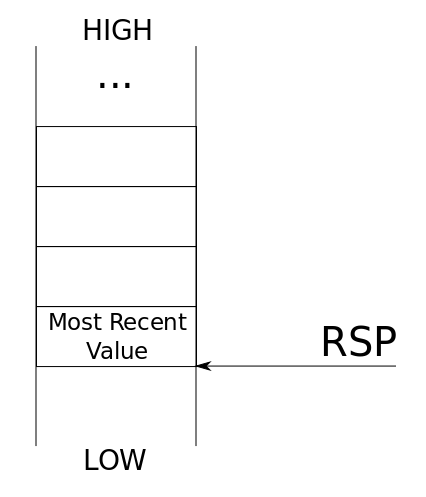
\includegraphics[height=.5\textheight]{stack}
    \hspace*{\fill}\hspace*{\fill}
\end{frame}

\begin{frame}[fragile]
\frametitle{Инструкции работы со стеком}
\begin{itemize}
    \item<1->\lstinline|pushq <src>| - уменьшает \emph{RSP}\\
    на 8 и сохраняет по полученному адресу \emph{src}
    \begin{itemize}
        \item<2->\lstinline|pushq $42|
        \item<3->\lstinline|pushq %RAX|
    \end{itemize}
\end{itemize}
\end{frame}

\begin{frame}
\frametitle{Инструкции работы со стеком}
    \hspace*{\fill}
    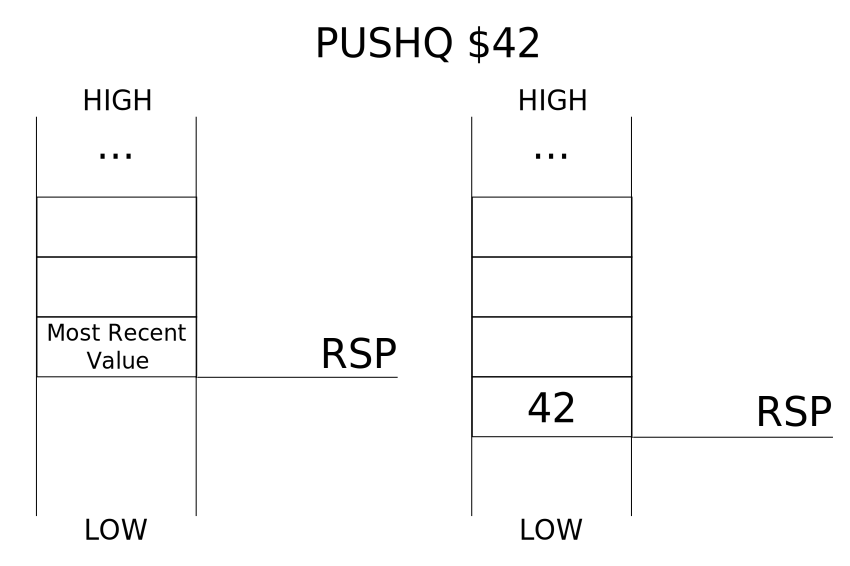
\includegraphics[height=.5\textheight]{pushq}
    \hspace*{\fill}\hspace*{\fill}
\end{frame}

\begin{frame}[fragile]
\frametitle{Инструкции работы со стеком}
\begin{itemize}
    \item<1->\lstinline|popq <dst>| - обратное действие\\
    к \emph{pushq}
    \begin{itemize}
        \item<2->\lstinline|popq %RAX|
    \end{itemize}
    \item<3->\lstinline|movq (%RSP), %RAX|
\end{itemize}
\end{frame}

\begin{frame}
\frametitle{Инструкции работы со стеком}
    \hspace*{\fill}
    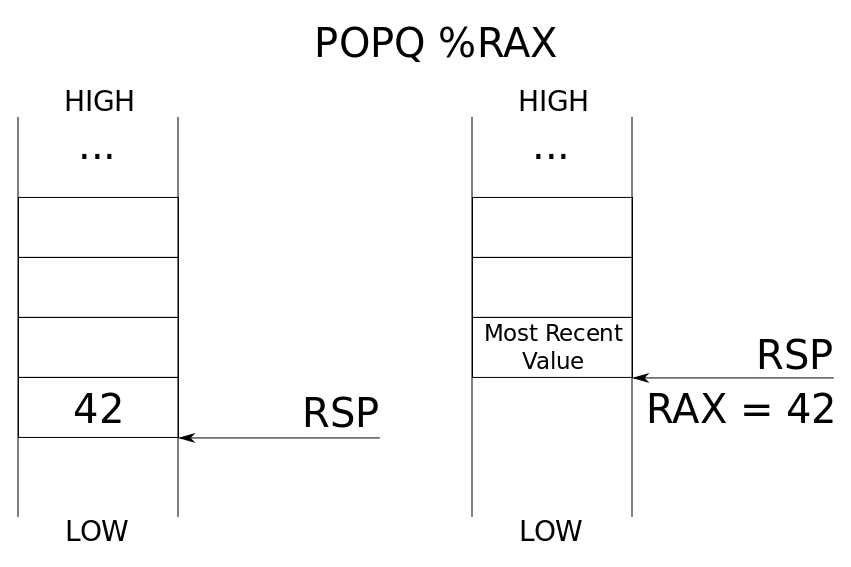
\includegraphics[height=.5\textheight]{popq}
    \hspace*{\fill}\hspace*{\fill}
\end{frame}

\begin{frame}[fragile]
\frametitle{Метки и переменные}
\begin{itemize}
    \item<1->Метка - просто имя для некоторого адреса:
    \begin{lstlisting}
	.data
value:
	.quad 42

	.text
add42:
	movq %rdi, %rax
	addq value, %rax
	retq
    \end{lstlisting}
\end{itemize}
\end{frame}

\begin{frame}[fragile]
\frametitle{Инструкции безусловного перехода}
\begin{itemize}
    \item<1-> Инструкции безусловного перехода изменяют\\
    значение регистра \emph{RIP}:
    \begin{itemize}
        \item<2->\lstinline|jmp <label>|
        \item<3->\lstinline|call <label>| - инструкция вызова функции
        \item<4->\lstinline|retq| - инструкция возврата из функции
    \end{itemize}
\end{itemize}
\end{frame}

\begin{frame}
\frametitle{Функции}
\begin{itemize}
    \item<1-> Функция:
    \begin{itemize}
        \item<2->функцию можно вызвать;
        \item<3->функция возвращает управление\\ \emph{вызвавшему коду}.
    \end{itemize}
\end{itemize}
\end{frame}

\begin{frame}
\frametitle{Вызов функции}
    \hspace*{\fill}
    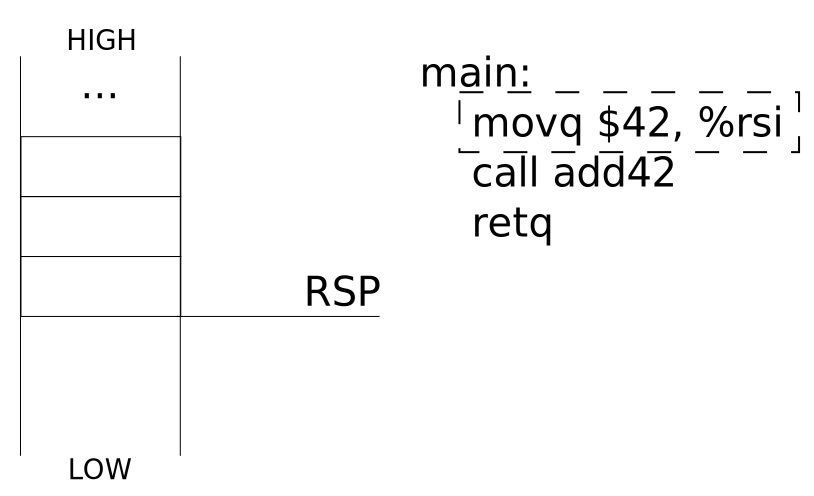
\includegraphics[height=.5\textheight]{call0}
    \hspace*{\fill}\hspace*{\fill}
\end{frame}

\begin{frame}
\frametitle{Вызов функции}
    \hspace*{\fill}
    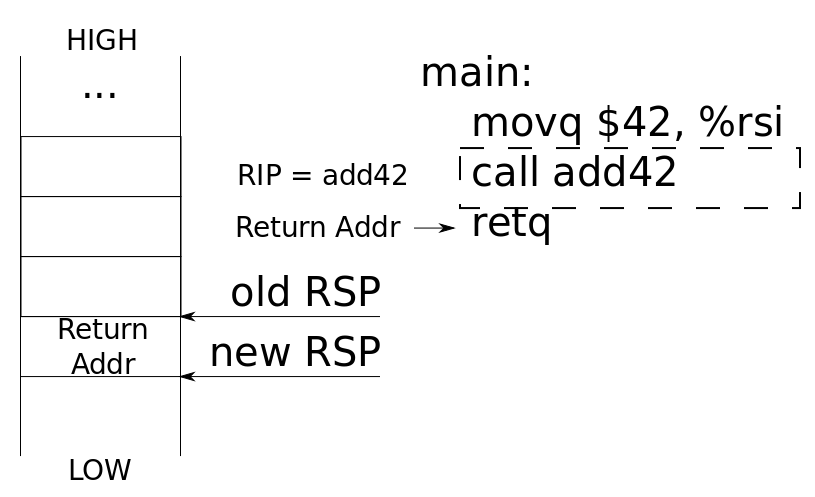
\includegraphics[height=.5\textheight]{call1}
    \hspace*{\fill}\hspace*{\fill}
\end{frame}

\begin{frame}
\frametitle{Флаговый регистр RFLAGS}
\begin{itemize}
    \item<1-> Флаговый регистр хранит флаги!
    \item<2-> Флаги регистра RFLAGS:
    \begin{itemize}
        \item \emph{ZF} - результат операции 0;
        \item \emph{CF} - произошло беззнаковое переполнение;
        \item \emph{OF} - произошло знаковое переполнение.
    \end{itemize}
\end{itemize}
\end{frame}

\begin{frame}[fragile]
\frametitle{Инструкции условного перехода}
\begin{itemize}
    \item<1->\lstinline|jcc <label>| - выполняет переход, если\\
    условие \emph{cc} истинно.
    \begin{itemize}
        \item<2->\lstinline|jz|, \lstinline|je| - проверяет, что $ZF = 1$;
        \item<2->\lstinline|jne|, \lstinline|jnz| - $ZF = 0$;
        \item<3->\lstinline|jg| - если "больше" (знаковый вариант);
        \item<3->\lstinline|jge| - "больше или равно" (знаковый вариант);
        \item<4->\lstinline|ja| - если "больше" (беззнаковый вариант);
        \item<4->\lstinline|jae| - "больше или равно" (беззнаковый вариант).
    \end{itemize}
\end{itemize}
\end{frame}

\begin{frame}[fragile]
\frametitle{Инструкции сравнения}
\begin{itemize}
    \item<1->Арифметические инструкции изменяют \\
    \emph{RFLAGS}\onslide<2->, но также изменяют свои аргументы!
    \item<3->Есть команды, которые выставляют\\
    флаги, но не изменяют свои аргументы:
    \begin{itemize}
        \item \lstinline|cmpq <src>, <dst>| - вычисляет разность \\
        $dst - src$ и выставляет флаги;
        \item т. е. \emph{cmpq} работает как \emph{subq}, \\
        но не изменяет \emph{dst}.
    \end{itemize}
\end{itemize}
\end{frame}

\begin{frame}[fragile]
\frametitle{Пример ветвления}
\begin{lstlisting}
max:
    movq %rdi, %rax
    cmpq %rsi, %rdi # rdi - rsi
    ja rdi_gt       # rdi - rsi > 0
    movq %rsi, %rax
rdi_gt:
    ret
\end{lstlisting}
\end{frame}
